%% Created by Yasuyuki SAITO, Department of Information Engineering.


%% 2016/01/13 Edit by Kouta ASAI, and Akira NEMOTO, Advanced Control and Information Engineering Course
%% 2017/12/07 Edit by by Shinichi OEDA, Department of Information Engineering.
%% 「★」マークが変更を加えた部分を表す

%% ★jsarticleに変更 fleqnで数式を左寄せにする
\documentclass[twocolumn, fleqn, uplatex]{jsarticle}

\usepackage{proceeding-DJ}
\usepackage{afterpage}
%% ★数式を使う人が多いと思うので
\usepackage{amsmath}
\usepackage{bm}
\usepackage{booktabs}
\usepackage{enumitem}
\usepackage{subcaption}


%% ★ヒラギノを使っている人向け
\usepackage[deluxe, expert]{otf}

% \makeatletter
% \long\def\@makecaption#1#2{%
%   \vskip\abovecaptionskip
%   \iftdir\sbox\@tempboxa{#1\hskip1zw#2}%
%     \else\sbox\@tempboxa{#1~ #2}%
%   \fi
%   \ifdim \wd\@tempboxa >\hsize
%     \iftdir #1\hskip1zw#2\relax\par
%     \else #1~ #2\relax\par\fi
%   \else
%   \global \@minipagefalse
%   \hbox to\hsize{\hfil\box\@tempboxa\hfil}%
% \fi
% \vskip\belowcaptionskip}
% \makeatother

\begin{document}

\pagestyle{empty}

%% 番号をつけるときはこのすぐ下の行を有効にして,番号を編集する.
%%\date{J--33}
%%所属をDJ以外にしたい場合は,styファイルを編集する.
\date{}
\titleJ{研究発表タイトル}
\titleE{The research title}
\authorJ{高専 太郎}
\authorE{Taro Kosen}
\abstract{The purpose of this study is ... \\
%
\hspace*{1zw} If you would like to start a new paragraph, you should use
``\texttt{\textbackslash hspace*\{1zw\}}''.}
% \keywords{The key word1 of the test for \LaTeXe \ template file, The key
% word2 of the test for \LaTeXe \ template file, The key word3 of the test
% for \LaTeXe \ template file}
\keywords{a a a a a a a a a a a a a a a a a a a a a a a a a a a a a a a
a a a a a a a a a a a a a a a a a a a a a a a a a a a a a a a a a a a a
a a a a a a a a a a a a a a a a a a a a a}
\maketitle

%% 現在ページの上部へのフロートの配置を抑制.
%% ここに記述しておくことで,最初のページの左段上部に図表を置かない.
\suppressfloats[t]


%%●●●●●●●●●●●●●●●
\section{はじめに}

文書領域の余白は,上28mm,下24mm,左右ともに20mm 空ける.

発表タイトルは16pt でセンタリングする.
%
フォントは,ゴシック体で,太字とする.
%
発表タイトルの下に10.5pt で1 行分空ける.

発表者氏名・所属は右端によせる.

abstract において途中で改行したくなったら,「\verb|\\|」を置く.
%
新しい段落では,\verb|\hspace*{1zw}| を置いて字下げをする.

本文領域は2 段組とし,段と段の間は8mm 空けることとする.

本文の文章は10.5pt で記述することとし,行間は1.5mm とする.

ページ番号(フッタ)は用いないこと.

通し番号(「DJ-1」など)は後から印刷するので記述しなくてよい.

\begin{figure}[t]
 \vspace*{\baselineskip}
 \begin{center}
  \includegraphics{test.eps}
  \caption{テスト画像.{\tt figure}環境では原則として{\tt [t]}を用いる.}
  \label{fig:test}
 \end{center}
\end{figure}


%%●●●●●●●●●
\section{章の例}

%%●●●●●●
\subsection{節の例その1}

章見出しは12pt,節見出しと項見出しは10.5pt を基本とする.
%
章番号とピリオドは半角のCentury フォントを用いることとし,ピリオドの後に
半角スペースを置いてから見出し語を書くこととする.

1.2 節がないのに,1.1 節を設けるのは論理的におかしいので注意すること.

英数字はいずれも半角文字を用いること.


%%●●●●●●
\subsubsection{項の例その1}

項は直前に空行を置かない.

%%●●●●●●
\subsubsection{項の例その2}

項は直前に空行を置かない.


%%●●●●●●
\subsection{節の例その2}

図のキャプションは図の下に表記すること(Fig.~\ref{fig:test}).
%
逆に,表のキャプションは表の上に表記すること(Table~\ref{tab:tableTest}).
%
いずれのキャプションも,図番号や表番号と説明文の間にコロン(:)は置かな
いこととし,意味のある見出しとなるように心がける.
%
当然,図番号や表番号は本文中で引用しなければならない(Fig.~\ref{fig:test2}).

\begin{figure}[htbp]
 \vspace*{\baselineskip}
 \begin{center}
  \includegraphics{test.eps}
  \caption{テスト画像.これは\texttt{[htbp]} を指定しているので,本文中
  に割り込む.}
  \label{fig:test2}
 \end{center}
\end{figure}

%%●●●●●●
\subsubsection{項の例その1}

項は直前に空行を置かない.

%%●●●●●●
\subsubsection{項の例その2}

図や表は,原則として\verb|figure|環境や\verb|table|環境において
\verb|[t]| を指定し,紙面の上部に配置する.
%
どうしても本文中に置きたい場合は,\verb|[h]| などを用いた上で,本文と間
を開けるために環境の冒頭にて\verb|\vspace*{\baselineskip}| を用いる.

\verb|dvipdfmx| コマンドでDVI ファイルから直接的にPDF ファイルを生成した
ときに図が含まれない場合,\verb|dvips| コマンドでPS ファイルに変換し,
\verb|ps2pdf| コマンドでPDF に変換するとよい.


%%●●●●●●●●●●●●●●●
\section{まとめ}

参考文献の見出しには章番号は振らないことに注意する.
%
当然,参考文献で挙げた文献は,本文中で必ず引用すること.

参考文献は9 pt とし,行間は1 mm で列挙する.
%
文献名を囲む記号の開始は「``」であり,「''」ではない.
%
向きに注意して確認を怠らないようにする.

各項目の区切りは半角のカンマとスペースとし,最後は半角のピリオドとする.

複数の文献を同時に引用するとき,2 つまでは半角カンマで区切る\cite{lit:一
朗, lit:太郎}.
%
3つ以上連続する場合は,ハイフンで最初と最後の文献番号を示す\cite{lit:華子,
lit:花子, lit:次郎}.
%
\LaTeXe では,連続している引用は\verb|\cite{ }| にカンマで区切って列挙す
るだけで自動的に範囲表示に変換される.
%
これは,不連続なものと連続しているものが混在していても,\verb|\cite{}|
の中の記述の順番が参考文献で挙げている順序通りでなくても,自動的に適切に
変換される\cite{lit:一朗, lit:次郎, lit:花子, lit:華子}.


\begin{table}[t]
 \begin{center}
  \caption{表のテスト}
  \label{tab:tableTest}
  \begin{tabular}{|c|c||c|}
   \hline
   入力1 & 入力2 & 出力 \\
   \whline
   0 & 0 & 0 \\
   0 & 1 & 1 \\
   1 & 0 & 1 \\
   1 & 1 & 0 \\
   \hline
  \end{tabular}
 \end{center}
\end{table}


\begin{thebibliography}{9}

 \bibitem{lit:一朗}
	 情報 一朗,
	 ``見出しに章番号をつけない'',
	 関東高専学会学会誌, Vol.5, pp.72-73, March 2004.

 \bibitem{lit:太郎}
	 高専 太郎,
	 ``参考文献は9pt,行間1mm で記述する'',
	 日本高専学会学会誌, Vol.19, pp.88-91, July 2005.

 \bibitem{lit:華子}
	 工学 華子,
	 ``囲む記号の開始記号の向きに注意'',
	 東日本高専学会学会誌, Vol.24, pp.54-55, Apr. 2003.

 \bibitem{lit:花子}
	 清見 花子,
	 ``区切りは半角のカンマとスペース'',
	 世界高専学会論文誌, Vol.34, pp.1006-1009, Oct. 2005.

 \bibitem{lit:次郎}
	 台東 次郎,
	 ``最後は半角ピリオド'',
	 宇宙高専学会技術報告, Vol.3, pp.12-15, Dec. 2006.

\end{thebibliography}

\end{document}
